\chapter{Categories}
\label{chap:categories}

\epigraph{
  And God saw every thing that he had made, and, \emph{behold}, it was
  very good.
}{---\textcite[Genesis 1:31]{god-1769}}

In this chapter we study categories in order to be able to study
functors and natural transformations, which are the basic concepts of
category theory. More interestingly, we see that, up to a point, the
types and functions of a functional programming language such as
Haskell yield a category which will allow us to relate category theory
to functional programming.

To motivate categories, consider the subset of Haskell types and
functions depicted by the diagram in Figure
\ref{fig:category-haskell}, excluding composite functions. More
specifically, as types, take the unit type, \texthaskell{()}, the
Boolean type, \texthaskell{Bool}, and the natural number type,
\texthaskell{Nat}\footnote{Note that Haskell does not have a natural
  number type by itself.}, and, as functions, take the
constants-as-functions \texthaskell{()}, \texthaskell{True},
\texthaskell{False}, and \texthaskell{Zero}, the functions
\texthaskell{Succ}, \texthaskell{isZero}, and \texthaskell{not}, the
identity functions, \texthaskell{id}, and composite functions such as
\texthaskell{not . True}.

\begin{figure}[htb]
  \begin{center}
    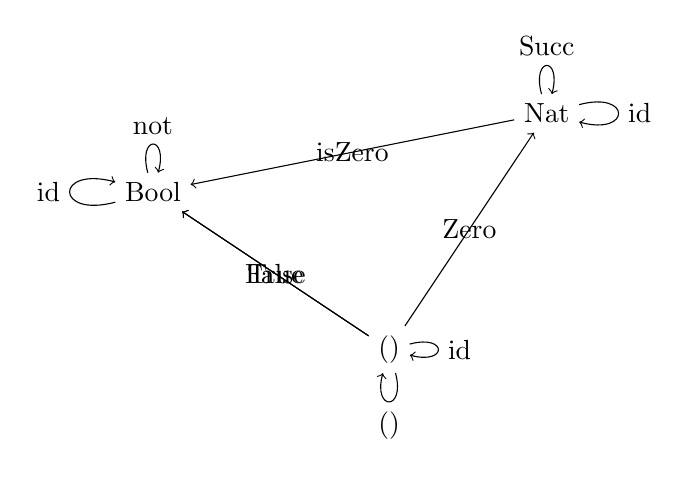
\begin{tikzpicture}[node distance=4cm]
      \node (bool) at (0,0)  {\texthaskell{Bool}};
      \node (nat)  at (5,1)  {\texthaskell{Nat}};
      \node (unit) at (3,-2) {\texthaskell{()}};

      \draw [->] (unit) to node        {\texthaskell{True}}  (bool);
      \draw [->] (unit) to node [swap] {\texthaskell{False}} (bool);

      \draw [->] (unit) to              node [swap] {\texthaskell{Zero}} (nat);
      \draw [->] (nat)  to [loop above] node        {\texthaskell{Succ}}  (nat);

      \draw [->] (unit) to [loop below] node {\texthaskell{()}} (unit);

      \draw [->] (bool) to [loop left]  node {\texthaskell{id}} (bool);
      \draw [->] (nat)  to [loop right] node {\texthaskell{id}} (nat);
      \draw [->] (unit) to [loop right] node {\texthaskell{id}} (unit);

      \draw [->] (bool) to [loop above] node        {\texthaskell{not}}    (bool);
      \draw [->] (nat)  to              node [swap] {\texthaskell{isZero}} (bool);
    \end{tikzpicture}
  \end{center}
  \caption{A subset of Haskell.}
  \label{fig:category-haskell}
\end{figure}

Now, observe that, according to the semantics of the language, some of
the functions, such as \texthaskell{isZero . Zero} and
\texthaskell{True}, are identical. Additionally, we could prove, for
instance, that \texthaskell{id . Succ = Succ = Succ . id}, which
exemplifies that identity functions are identities for the composition
of functions, which is associative.

In terms of category theory, the types and functions of this subset of
Haskell represent the objects and morphisms of a category,
respectively, and the statement that composition of functions is
associative and has identities means that we are in fact dealing with
a category.

In the remainder of this chapter, we define the concepts of category
and commutative diagram, and give some examples of categories,
including the category of sets and functions. In addition, we describe
categories of types and functions for Haskell and Agda.

\section{Categories}
\label{sec:categories}

We begin with the concept of category, which will be found everywhere
in our development.

\begin{definition}
  \label{def:category}

  %% \parencites[4--5]{awodey-2010}[7--8, 289]{maclane-1998}

  A category \cat{C} consists of:
  \begin{itemize}
  \item
    Objects $a$, $b$, $c$, ...

  \item
    Morphisms or arrows $f$, $g$, $h$, ...

  \item
    For each morphism $f$, domain and codomain objects $a = \dom(f)$
    and $b = \cod(f)$, respectively. We then write $f: a \to b$.

  \item
    For each object $a$, an identity morphism $\idO{a}: a \to a$.

  \item
    For each pair of morphisms $f: a \to b$ and $g: b \to c$, a
    composite morphism $g \comp f: a \to c$. That is, for each pair of
    morphisms $f$ and $g$ with $\cod(f) = \dom(g)$, a composite
    morphism $g \comp f: \dom(f) \to \cod(g)$. We may then draw a
    diagram like that of Figure \ref{fig:category-composition}.

    \begin{figure}[htb]
      \begin{center}
        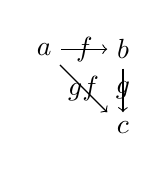
\begin{tikzpicture}
          \node (a)              {$a$};
          \node (b) [right of=a] {$b$};
          \node (c) [below of=b] {$c$};

          \draw [->] (a) to node        {$f$}         (b);
          \draw [->] (b) to node        {$g$}         (c);
          \draw [->] (a) to node [swap] {$g \comp f$} (c);
        \end{tikzpicture}
      \end{center}
      \caption{Composition of morphisms.}
      \label{fig:category-composition}
    \end{figure}

    Composition of morphisms associates to the right. Therefore, for
    all morphisms $f: a \to b$, $g: b \to c$, and $h: c \to d$, $h
    \comp g \comp f$ denotes $h \comp (g \comp f)$.

  \end{itemize}
  The category is subject to the following axioms:
  \begin{itemize}
  \item
    For all morphisms $f: a \to b$, $g: b \to c$, and $h: c \to d$,
    \begin{equation}
      \label{eq:category-associativity}
      h \comp (g \comp f) = h \comp g \comp f = (h \comp g) \comp f
      \text{,}
    \end{equation}
    that is, composition of morphisms is associative or, equivalently,
    the diagram in Figure \ref{fig:category-associativity} is
    commutative.

  \item
    For all morphisms $f: a \to b$,
    \begin{equation}
      \label{eq:category-identity}
      \idO{b} \comp f = f = f \comp \idO{a}
      \text{,}
    \end{equation}
    that is, identity morphisms are identities for the composition of
    morphisms or, equivalently, the diagram in Figure
    \ref{fig:category-identity} is commutative.

    \begin{figure}[htb]
      \begin{center}
        \begin{subfigure}[t]{0.45\linewidth}
          \begin{center}
            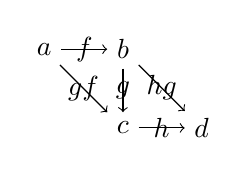
\begin{tikzpicture}
              \node (a)              {$a$};
              \node (b) [right of=a] {$b$};
              \node (c) [below of=b] {$c$};
              \node (d) [right of=c] {$d$};

              \draw [->] (a) to node        {$f$} (b);
              \draw [->] (b) to node        {$g$} (c);
              \draw [->] (c) to node [swap] {$h$} (d);

              \draw [->] (a) to node [swap] {$g \comp f$} (c);
              \draw [->] (b) to node        {$h \comp g$} (d);
            \end{tikzpicture}
          \end{center}
          \caption{The associativity axiom.}
          \label{fig:category-associativity}
        \end{subfigure}
        \begin{subfigure}[t]{0.45\linewidth}
          \begin{center}
            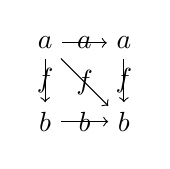
\begin{tikzpicture}
              \node (a1)               {$a$};
              \node (a2) [right of=a1] {$a$};
              \node (b1) [below of=a1] {$b$};
              \node (b2) [right of=b1] {$b$};

              \draw [->] (a1) to node        {$\idO{a}$} (a2);
              \draw [->] (b1) to node [swap] {$\idO{b}$} (b2);

              \draw [->] (a1) to node [swap] {$f$} (b1);
              \draw [->] (a1) to node        {$f$} (b2);
              \draw [->] (a2) to node        {$f$} (b2);
            \end{tikzpicture}
          \end{center}
          \caption{The identity axiom.}
          \label{fig:category-identity}
        \end{subfigure}
      \end{center}
      \caption{Axioms for categories.}
      \label{fig:category-axioms}
    \end{figure}

  \end{itemize}

\end{definition}

\epigraph{
  ``And what is the use of a book without pictures or conversations?''
}{---\textcite[13]{carroll-2004}}

\begin{definition}
  \label{def:commutative-diagram}

  %% \parencites[8]{maclane-1998}[434--435]{poigne-1992}

  We often use diagrams consisting of objects and morphisms of a
  category, like those of Figures \ref{fig:category-composition} and
  \ref{fig:category-axioms}. Such a diagram in a category \cat{C} is
  said to be commutative, or to commute, when, for each pair of
  objects $a$ and $b$, any two paths leading from $a$ to $b$ yield, by
  composition, equal morphisms from $a$ to $b$. For instance, if we
  say that the diagram in Figure \ref{fig:commutative-square} is
  commutative, we mean that
  \begin{equation*}
    g' \comp f' = g \comp f
    \text{.}
  \end{equation*}
  In this way, ``commutative diagrams are just a convenient way to
  visualize equalities of morphisms'' \parencite[434]{poigne-1992}.

  \begin{figure}[htb]
    \begin{center}
      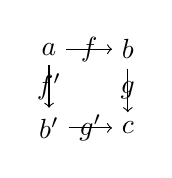
\begin{tikzpicture}
        \node (a)               {$a$};
        \node (b)  [right of=a] {$b$};
        \node (b') [below of=a] {$b'$};
        \node (c)  [below of=b] {$c$};

        \draw [->] (a)  to node        {$f$}  (b);
        \draw [->] (b)  to node        {$g$}  (c);
        \draw [->] (a)  to node [swap] {$f'$} (b');
        \draw [->] (b') to node [swap] {$g'$} (c);
      \end{tikzpicture}
    \end{center}
    \caption{A commutative square.}
    \label{fig:commutative-square}
  \end{figure}

\end{definition}

\begin{remark}
  \label{re:commutative-diagram}

  %% \parencite[434--435]{poigne-1992}

  Moreover, commutative diagrams are closed under composition of
  diagrams in that a diagram commutes if all its subdiagrams commute.
  For example, if we say that the inner triangles of the diagram in
  Figure \ref{fig:commutative-triangles} commute, then the outer
  diagram commutes as well, that is, if
  \begin{equation*}
    f' = h \comp f
    \quad
    \text{and}
    \quad
    g = g' \comp h
    \text{,}
  \end{equation*}
  then
  \begin{equation*}
    g' \comp f' = g' \comp h \comp f = g \comp f
    \text{.}
  \end{equation*}

  \begin{figure}[htb]
    \begin{center}
      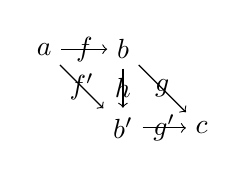
\begin{tikzpicture}
        \node (a)                {$a$};
        \node (b)  [right of=a]  {$b$};
        \node (b') [below of=b]  {$b'$};
        \node (c)  [right of=b'] {$c$};

        \draw [->] (a)  to node        {$f$}  (b);
        \draw [->] (a)  to node [swap] {$f'$} (b');
        \draw [->] (b)  to node        {$g$}  (c);
        \draw [->] (b)  to node        {$h$}  (b');
        \draw [->] (b') to node [swap] {$g'$} (c);
      \end{tikzpicture}
    \end{center}
    \caption{Commutative triangles.}
    \label{fig:commutative-triangles}
  \end{figure}

\end{remark}

As examples, we consider some common categories, including the empty
category, the trivial category, discrete categories, the category of
sets and functions, which is the motivating example of category
theory, monoids, which help to better understand the idea of sets with
structure as categories, and deductive systems, which is an
interesting change of perspective.

\begin{example}
  \label{ex:category-trivial}

  %% \parencites[7--8]{awodey-2010}[10--11]{maclane-1998}[422]{poigne-1992}

  The empty category, \catbf{0}, has neither objects nor morphisms. It
  looks like, well, nothing. The trivial category, \catbf{1}, has one
  object and one (identity) morphism. It looks like the diagram in
  Figure \ref{fig:category-1}, which is a diagram of a category,
  excluding the identity morphisms. The category \catbf{2} has two
  objects, two identity morphisms and one (non-identity) morphism
  which looks like the morphism of the category in Figure
  \ref{fig:category-2}. And the category \catbf{3} has three objects,
  three identity morphisms, and three (non-identity) morphisms which
  look like the morphisms of the category in Figure
  \ref{fig:category-3}. In each case, there is only one way to define
  composition of morphisms, and the axioms for categories obviously
  hold.

  \begin{figure}[htb]
    \begin{center}
      \begin{subfigure}[t]{.3\linewidth}
        \begin{center}
          \begin{tikzpicture}
            \node (a) {$a$};
          \end{tikzpicture}
        \end{center}
        \caption{The category \catbf{1}.}
        \label{fig:category-1}
      \end{subfigure}
      \begin{subfigure}[t]{.3\linewidth}
        \begin{center}
          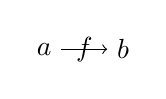
\begin{tikzpicture}
            \node (a)              {$a$};
            \node (b) [right of=a] {$b$};

            \draw [->] (a) to node {$f$} (b);
          \end{tikzpicture}
        \end{center}
        \caption{The category \catbf{2}.}
        \label{fig:category-2}
      \end{subfigure}
      \begin{subfigure}[t]{.3\linewidth}
        \begin{center}
          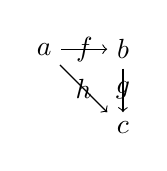
\begin{tikzpicture}
            \node (a)              {$a$};
            \node (b) [right of=a] {$b$};
            \node (c) [below of=b] {$c$};

            \draw [->] (a) to node        {$f$} (b);
            \draw [->] (b) to node        {$g$} (c);
            \draw [->] (a) to node [swap] {$h$} (c);
          \end{tikzpicture}
        \end{center}
        \caption{The category \catbf{3}.}
        \label{fig:category-3}
      \end{subfigure}
    \end{center}
    \caption{}
    \label{fig:category-trivial}
  \end{figure}

\end{example}

\begin{example}
  \label{ex:category-discrete}

  %% \parencite[8, 11]{maclane-1998}[422]{poigne-1992}

  A discrete category is a category whose only morphisms are the
  identity morphisms. Given a set $A$, we get a discrete category
  \cat{C} in which the objects are the elements of $A$ and the
  morphisms are the identity morphisms, one for each $x \in A$, which
  are uniquely determined by the identity axiom. A discrete category
  is so determined by its objects, which correspond exactly to its
  identity morphisms.

\end{example}

\begin{example}
  \label{ex:category-set}

  %% \parencite[8--9]{maclane-1998}

  \set is the category of sets and functions. Its objects are sets
  $A$, $B$, $C$, ..., and its morphisms are functions $f$, $g$, $h$,
  ... Each function $f: A \to B$ is composed of a domain $A =
  \dom(f)$, a codomain or range $B = \cod(f)$, and a rule which
  assigns to each element $x \in A$ an element $f(x) \in B$. For each
  set $A$, there is an identity function $\idO{A}: A \to A$ such that,
  for all $x \in A$,
  \begin{equation}
    \label{eq:set-identity}
    \idO{A}(x) = x
    \text{,}
  \end{equation}
  and, for each pair of morphisms $f: A \to B$ and $g: B \to C$, there
  is a composite function $g \comp f: A \to C$ such that, for all $x
  \in A$,
  \begin{equation}
    \label{eq:set-composition}
    (g \comp f)(x) = g(f(x))
    \text{.}
  \end{equation}
  Now, let us prove that this is a category. In the first place, we
  prove that the associativity axiom holds for \set. Given functions
  $f: A \to B$, $g: B \to C$, and $h: C \to D$, then, for all $x \in
  A$:
  \begin{steps}
    \stepm{(h \comp g \comp f)(x)}
      \eqby{\eqref{eq:set-composition}}
    \stepm{h((g \comp f)(x))}
      \eqby{\eqref{eq:set-composition}}
    \stepm{h(g(f(x)))}
      \eqby{\eqref{eq:set-composition}}
    \stepm{(h \comp g)(f(x))}
      \eqby{\eqref{eq:set-composition}}
    \stepm{((h \comp g) \comp f)(x)}
  \end{steps}
  In the second place, we prove that the identity axiom holds for
  \set. Given a function $f: A \to B$, then, for all $x \in A$:
  \begin{steps}
    \stepm{(\idO{B} \comp f)(x)}
      \eqby{\eqref{eq:set-composition}}
    \stepm{\idO{B}(f(x))}
      \eqby{\eqref{eq:set-identity}}
    \stepm{f(x)}
      \eqby{\eqref{eq:set-identity}}
    \stepm{f(\idO{A}(x))}
      \eqby{\eqref{eq:set-composition}}
    \stepm{(f \comp \idO{A})(x)}
  \end{steps}

  \begin{remark}
    \label{re:foundations}

    %% \parencite[12, 21]{maclane-1998}

    %% \parencites[§ 1.8]{awodey-2010}[§ I.6]{maclane-1998}

    To some extent, we are considering the objects and morphisms of
    \set to be the sets of all sets and all functions, respectively,
    which would lead to a paradox such as the set of all sets not
    members of themselves. For this reason, we ought to assume, for
    instance, that there is a big enough set, the universe, and take
    the objects of \set to be the sets which are members of the
    universe, that is, small sets. However, we shall not go into
    detail about mathematical foundations of category
    theory\footnote{For a full account on mathematical foundations of
      category theory, see \parencites[§ 1.8]{awodey-2010}[§
        I.6]{maclane-1998}.}.

  \end{remark}

\end{example}

\begin{example}
  \label{ex:category-monoid}

  %% \parencites[11]{maclane-1998}[422]{poigne-1992}

  %% \parencite[21]{adamek-et-al-2006}

  A monoid is a category with just one object. A monoid is thus
  determined by its morphisms, its identity morphism, and its rule for
  the composition of morphisms. A monoid may then be described as a
  usual monoid, that is, as a set (of morphisms) that is closed under
  an associative binary operation which has an identity (morphism).
  More formally, given a category \cat{C} with just one object $a$, we
  get a usual monoid $C = (\catM{C}, \comp, \idO{a})$ where the
  elements of \catM{C} are the morphisms of \cat{C}. Conversely, given
  a usual monoid $M = (M, *, e)$, we get a category \cat{M} with just
  one object $M$, morphisms the elements of $M$, composition $*$ and
  identity morphism $e$.

  \begin{remark}
    \label{re:category-mon}

    %% \parencite[420--421]{poigne-1992}

    \catbf{Mon} is the category of monoids and monoid homomorphisms,
    which we shall not describe here. This category is just one
    example of the fact that any notion of sets with structure
    together with morphisms that preserve that structure define a
    category.

  \end{remark}

\end{example}

\begin{example}
  \label{ex:category-deductive-system}

  %% \parencite[Example 1.1.14]{pierce-1991}

  %% \parencite[§ 9.1]{poigne-1992}

  We can look at categories as deductive systems with objects formulas
  and morphisms deductions. In this way, domains and co\-do\-mains are
  premises and conclusions, respectively. A morphism is thus a proof
  of the fact that its codomain is deducible from its domain. In
  particular, identity morphisms are instances of the reflexivity
  axiom, and composition of morphisms is a rule of inference asserting
  that deductions are transitive. Note that this is just a change of
  vocabulary.

\end{example}

Before we move on, let us revisit the motivating example of the subset
of Haskell, which we shall complete in the following section.

\begin{example}
  \label{ex:category-haskell}

  %% \parencites[Example 1.1.15]{pierce-1991}[7--11]{pitt-1986}

  The motivating example of the subset of Haskell corresponds to a
  category. Its objects are the types \texthaskell{()},
  \texthaskell{Bool}, and \texthaskell{Nat}, and its morphisms are the
  constants-as-functions
  \begin{itemize}
  \item
    \texthaskell{() :: () -> ()},

  \item
    \texthaskell{True} and \texthaskell{False :: () -> Bool}, and

  \item
    \texthaskell{Zero :: () -> Nat},

  \end{itemize}
  the functions
  \begin{itemize}
  \item
    \texthaskell{Succ :: Nat -> Nat},

  \item
    \texthaskell{not :: Bool -> Bool}, and

  \item
    \texthaskell{isZero :: Bool -> Bool},

  \end{itemize}
  the identity functions, \texthaskell{id}, and composite functions
  \begin{itemize}
  \item
    \texthaskell{not . True}, \texthaskell{not . (not . True) :: () -> Bool}, ...,

  \item
    \texthaskell{Succ . Zero}, \texthaskell{Succ . (Succ . Zero) :: () -> Nat}, ...,

  \item
    \texthaskell{isZero . Zero}, \texthaskell{isZero . (Succ . Zero) :: () -> Bool}, ...,

  \item
    and so on.

  \end{itemize}
  We shall not prove the associativity and identity axioms yet, but,
  evidently, this subset of Haskell is a category. What would result
  if we considered all of Haskell?

\end{example}

\section{A Category for Haskell}
\label{sec:category-haskell}

Having described a subset of Haskell types and functions as a
category, let us now construct a general category for Haskell.
Intuitively, if we keep adding types and functions to the category of
Example \ref{ex:category-haskell}, we get what we want. But we have to
be careful because there are some features of Haskell which we cannot
omit.

In a nutshell, \hask is the category of Haskell types and functions.
As expected, the objects of this category are Haskell types, that is,
nullary type constructors or type expressions with kind
\texthaskell{*}\footnote{In Haskell, type expressions are classified
  into different kinds, which are like types of types. See
  \parencite[§ 4.1.1]{peytonjones-2003}.}. For instance, the Boolean
type, \texthaskell{Bool}:
\begin{codehaskell}
data Bool = False | True
\end{codehaskell}
The natural number type, \texthaskell{Nat}:
\begin{codehaskell}
data Nat = Zero | Succ Nat
\end{codehaskell}
The integer types, \texthaskell{Int} and \texthaskell{Integer}, the
floating-point number types, \texthaskell{Float} and
\texthaskell{Double}, the Unicode character type, \texthaskell{Char},
lists of types such as \texthaskell{[Bool]} and \texthaskell{[Nat]},
\texthaskell{Maybe} types such as \texthaskell{Maybe Bool} and
\texthaskell{Maybe Nat}:
\begin{codehaskell}
data Maybe a = Nothing | Just a
\end{codehaskell}
But not \texthaskell{[]} and \texthaskell{Maybe}, which are unary type
constructors or type expressions with kind \texthaskell{* -> *}.

However, Haskell types have bottom. For example:
\begin{codehaskell}
undefined :: a
undefined = undefined
\end{codehaskell}
As a consequence, values of type \texthaskell{Bool} include
\texthaskell{True} and \texthaskell{False}, but also
\texthaskell{undefined}, values of type \texthaskell{Nat} include
\texthaskell{Zero} and \texthaskell{Succ Zero}, but also
\texthaskell{undefined}, and so forth, which is a
difficulty\footnote{See
  \url{http://www.haskell.org/haskellwiki/Hask}.}. For this reason, by
``Haskell types'' we mean ``Haskell types without bottom values,''
which is why \hask is sometimes considered a platonic category.

As anticipated, the morphisms of \hask are Haskell functions. For
instance, \texthaskell{not}:
\begin{codehaskell}
not :: Bool -> Bool
not False = True
not True  = False
\end{codehaskell}
And \texthaskell{isZero}:
\begin{codehaskell}
isZero :: Nat -> Bool
isZero Zero = True
isZero _    = False
\end{codehaskell}

For each type \texthaskell{a}, there is an identity function,
\texthaskell{id}:
\begin{codehaskell}
id :: a -> a
id x = x
\end{codehaskell}
And, for each pair of morphisms \texthaskell{f :: a -> b} and
\texthaskell{g :: b -> c}, there is a composite function,
\texthaskell{g . f}:
\begin{codehaskell}
infixr 9 .

(.) :: (b -> c) -> (a -> b) -> a -> c
g . f = \x -> g (f x)
\end{codehaskell}

As a result, the associativity axiom becomes, whenever it makes sense:
\begin{codehaskell}
h . (g . f) = h . g . f = (h . g) . f
\end{codehaskell}
And the identity axiom becomes, for all functions \texthaskell{f :: a
  -> b}:
\begin{codehaskell}
id . f = f = f . id
\end{codehaskell}
Both axioms follow immediately from rewriting using definitions. In
the first place:
\begin{steps}
  \steph{(h . (g . f)) x}
    \eqbydefh{(.)}
  \steph{h ((g . f) x)}
    \eqbydefh{(.)}
  \steph{h (g (f x))}
    \eqbydefh{(.)}
  \steph{(h . g) (f x)}
    \eqbydefh{(.)}
  \steph{((h . g) . f) x}
\end{steps}
In the second place:
\begin{steps}
  \steph{(id . f) x}
    \eqbydefh{(.)}
  \steph{id (f x)}
    \eqbydefh{id}
  \steph{f x}
    \eqbydefh{id}
  \steph{f (id x)}
    \eqbydefh{(.)}
  \steph{(f . id) x}
\end{steps}

From now on, we shall use \hask as described above as Haskell's
category\footnote{Note that this is not an attempt to answer the
  question of Haskell's category.}.

\section{A Category for Agda}
\label{sec:category-agda}

In Agda, types are called sets and there is an infinite hierarchy of
universes \textagda{Set₀}, \textagda{Set₁}, \textagda{Set₂}, ..., such
that \textagda{Set₀} is of type \textagda{Set₁}, \textagda{Set₁} is of
type \textagda{Set₂}, and so on. The first universe, \textagda{Set₀}
or \textagda{Set}, which is called the universe of small types, and
the second universe, \textagda{Set₁}, will be the only universes
necessary for our development \parencite[§ 2.1]{sicardramirez-2014}.

Let us now construct a category analogous to \hask, the category of
Haskell types and functions, in Agda. The objects of this category are
small types, that is, types of type \textagda{Set}. For example, the
Boolean type, \textagda{Bool}:
\begin{codeagda}
data Bool : Set where
  true  : Bool
  false : Bool
\end{codeagda}
And the natural number type, \textagda{Nat}:
\begin{codeagda}
data ℕ : Set where
  zero : ℕ
  succ : ℕ → ℕ
\end{codeagda}
And the morphisms of this category are functions between small types.
For instance, \textagda{not}:
\begin{codeagda}
not : Bool → Bool
not true  = false
not false = true
\end{codeagda}

For each small type \textagda{A}, there is an identity function
defined as follows:
\begin{codeagda}
id : {A : Set} → A → A
id x = x
\end{codeagda}
And, for each pair of functions \textagda{f : A → B} and \textagda{g:
  B → C}, there is a composite function, \textagda{g ∘ f}:
\begin{codeagda}
infixr 9 _∘_

_∘_ : {A B C : Set} → (B → C) → (A → B) → A → C
g ∘ f = λ x → g (f x)
\end{codeagda}
For both of these definitions, see the module \module{Abel.Function}.

Unlike in Haskell, the associativity and identity axioms for this
category are declared and proved in Agda (see the module
\module{Abel.Function.Category}):
\begin{codeagda}
associativity : {A B C D : Set} {f : A → B} {g : B → C} {h : C → D}
                (x : A) → (h ∘ g ∘ f) x ≡ ((h ∘ g) ∘ f) x
associativity _ = refl

identity : {A B : Set} {f : A → B}
           (x : A) → (id ∘ f) x ≡ f x × (f ∘ id) x ≡ f x
identity _ = refl , refl
\end{codeagda}

From now on, we shall use this category as Agda's
category\footnote{Note that this is not an attempt to answer the
  question of Agda's category.} and call it \agda.

\section{References}
\label{sec:categories-references}

The definition of category is based on
\parencites[4--5]{awodey-2010}[7--8, 289]{maclane-1998}. We defined
categories directly, but they can be defined in many ways. For
instance, \textcite{eilenberg-maclane-1945} defined them as aggregates
of objects and mappings, and \textcite{maclane-1998} did it in terms
of metacategories and in terms of sets, as sets of objects and arrows.
Other ways include defining them as sets of objects and morphisms,
just a set of morphisms, and in terms of collections of morphisms or
hom-sets.

The definition of commutative diagram is based on
\parencites[8]{maclane-1998}[434--435]{poigne-1992}, but almost any
reference on category theory contains an equivalent definition.
Additionally, the examples of categories are based on
\parencites[7--8]{awodey-2010}[8--12, 21]{maclane-1998}[Example
  1.1.14]{pierce-1991}[§ 1.2.2]{poigne-1992}.

Finally, the motivating example of the subset of Haskell is based on
\parencites[Example 1.1.15]{pierce-1991}[7--11]{pitt-1986}. For more
information about categories in Haskell, including \hask, see
\parencites[74]{elkins-2009}[49--51]{yorgey-2009}.

\clearemptydoublepage
